%=====================================================
\begin{frame}{2.1.4. Данные по вопросам, включенным в блок ``Декларируемый уровень доверия к коллегам'' }

\tiny


\begin{tabular}{lccl}

 & Да & Нет &\\

\begin{minipage}{0.62\textwidth}
Б10. ``С Вашей точки зрения, большинству коллег в Вашей образовательной организации можно доверять (доверие - уверенность в том, что, если Вы сказали коллеге о своих проблемах или ошибках, то эта информация не будет использована Вам во вред)?''
\end{minipage}
& \valBADyesNumA & \valBADnoNumA &
\begin{minipage}{1.55cm}
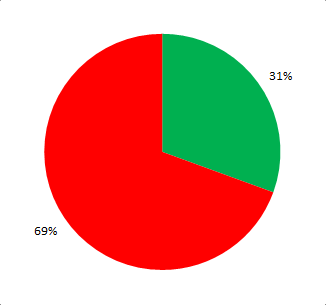
\includegraphics[width=1.5cm, height=1.5cm]{diag.png}
\end{minipage}
\\[0.5cm]

\begin{minipage}{0.62\textwidth}
Б13.  ``Есть ли у Вас профессиональные задачи, решение которых требует знакомства с опытом работы других педагогов (преподавателей, воспитателей) Вашей образовательной организации?''
\end{minipage}
& \valBADyesNumB & \valBADnoNumB &
\begin{minipage}{1.55cm}
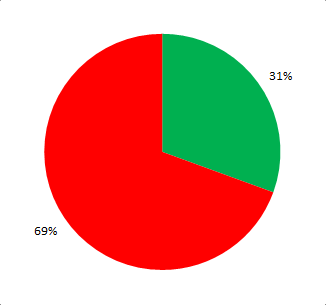
\includegraphics[width=1.5cm, height=1.5cm]{diag.png}
\end{minipage}
\\[0.5cm]

\begin{minipage}{0.62\textwidth}
Б14. ``Считаете ли Вы полезным и правильным посещение педагогами (преподавателями, воспитателями)  занятий и мероприятий (не открытых, т.е. специально не подготовленных), проводимых другими?''
\end{minipage}
& \valBADyesNumC & \valBADnoNumC &
\begin{minipage}{1.55cm}
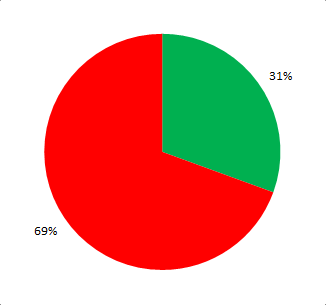
\includegraphics[width=1.5cm, height=1.5cm]{diag.png}
\end{minipage}
\\[0.5cm]

\begin{minipage}{0.62\textwidth}
Б25. ``Как Вам кажется, нравится ли педагогам (преподавателям, воспитателям) то, что Вы посещаете их занятия и мероприятия?''
\end{minipage}
& \valBADyesNumD & \valBADnoNumD &
\begin{minipage}{1.55cm}
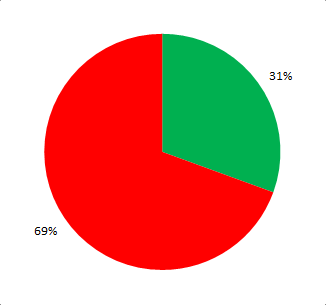
\includegraphics[width=1.5cm, height=1.5cm]{diag.png}
\end{minipage}
\\[0.5cm]

\begin{minipage}{0.62\textwidth}
Б30. ``Спокойно ли Вам коллеги предоставляют свой кабинет (группу), оборудование для проведения урока (занятия или мероприятия)?''
\end{minipage}
& \valBADyesNumE & \valBADnoNumE &
\begin{minipage}{1.55cm}
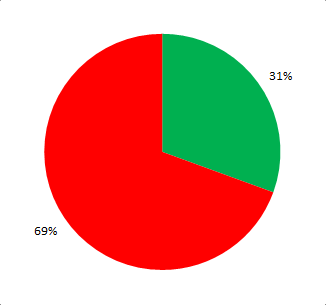
\includegraphics[width=1.5cm, height=1.5cm]{diag.png}
\end{minipage}

\end{tabular}

\end{frame}


